\RequirePackage{plautopatch}%新おまじない
\RequirePackage[l2tabu, orthodox]{nag}%おまじない

%test_ver

\documentclass[a4paper,12pt,twoside,openright,uplatex,dvipdfmx,titlepage]{jsbook}
\usepackage{graphicx}
\usepackage{epic,eepic}
\usepackage{amsmath}
\usepackage{amssymb}
\usepackage{txfonts}
\usepackage{jsreport}
\usepackage{osuka-sugimoto-lab}




%%%%%%%%%%%%%%%%%%%%%%%%%%%%%%%%%%%%%%%%%%%%%%%%%%%%%%%%%%%%%%%%%%%%%%%
\begin{document}
%%%%%%%%%%%%%%%%%%%%%%%%%%%%%%%%%%%%%%%%%%%%%%%%%%%%%%%%%%%%

%タイトル

\begin{titlepage}
  \centering

%\vspace*{3cm}
{\Large 令和○年度 --論文} 
\vspace{1cm} \\
 {\Large 題目} \\
{\huge \textbf{学士,修士認定のための\protect\\論文テンプレートはこちら}}\\ 
\vspace{5cm}

  

指導教員 \vspace{0.1cm} \\
{\Large -- -- 教授} \\
{\Large -- -- 准教授} \\
{\Large -- -- 助教} \\
\vspace{1cm}
{\Large 大阪大学大学院 工学研究科 機械工学専攻}\\
  {\Large 学籍番号 --------} 
  \vspace{0.5cm} \\
  {\LARGE -- --}
\vspace{2.5cm}
  
 
  \vfill
  

    {\Large 20--年2月--日}

   
  \vfill
  
 
   
  \end{titlepage}
%%%%%%%%%%%%%%%%%%%%%%%%%%%%%%%%%%%%%%%%%%%%%%%%%%%%%%%%%%%%
%
%
%前書き
\frontmatter



%%%%%%%%%%%%%%%%%%%%%%%%%%%%%%%%%%%%%%%%%%%%%%%%%%%%%%%%%%%%
%概要
\chapter*{\LARGE 概要}
\thispagestyle{empty}

ここに概要を書こう.






%%%%%%%%%%%%%%%%%%%%%%%%%%%%%%%%%%%%%%%%%%%%%%%%%%%%%%%%%%%

\newpage

%
%目次
\setcounter{page}{3}%ページ番号のリセット,概要からページを数えずに,目次からページ番号を始めたい場合は1にする
\tableofcontents
\newpage
\listoffigures
\newpage
%
%本文
\mainmatter

%%%%%%%%%%%%%%%%%%%%%%%%%%%%%%%%%%%%%%%%%%%%%%%%%%%%%%%%%%%%
%%%%%%%%%%%%%%%%%%%%%%%%%%%%%%%%%%%%%%%%%%%%%%%%%%%%%
% 緒言
%%%%%%%%%%%%%%%%%%%%%%%%%%%%%%%%%%%%%%%%%%%%%%%%%%%%%


緒言を書こう~\cite{bibtest}.

図の参照テスト Fig.~\ref{fig:test}.%reffig使うと太字になります


\begin{figure}[tb]
    \centering 
     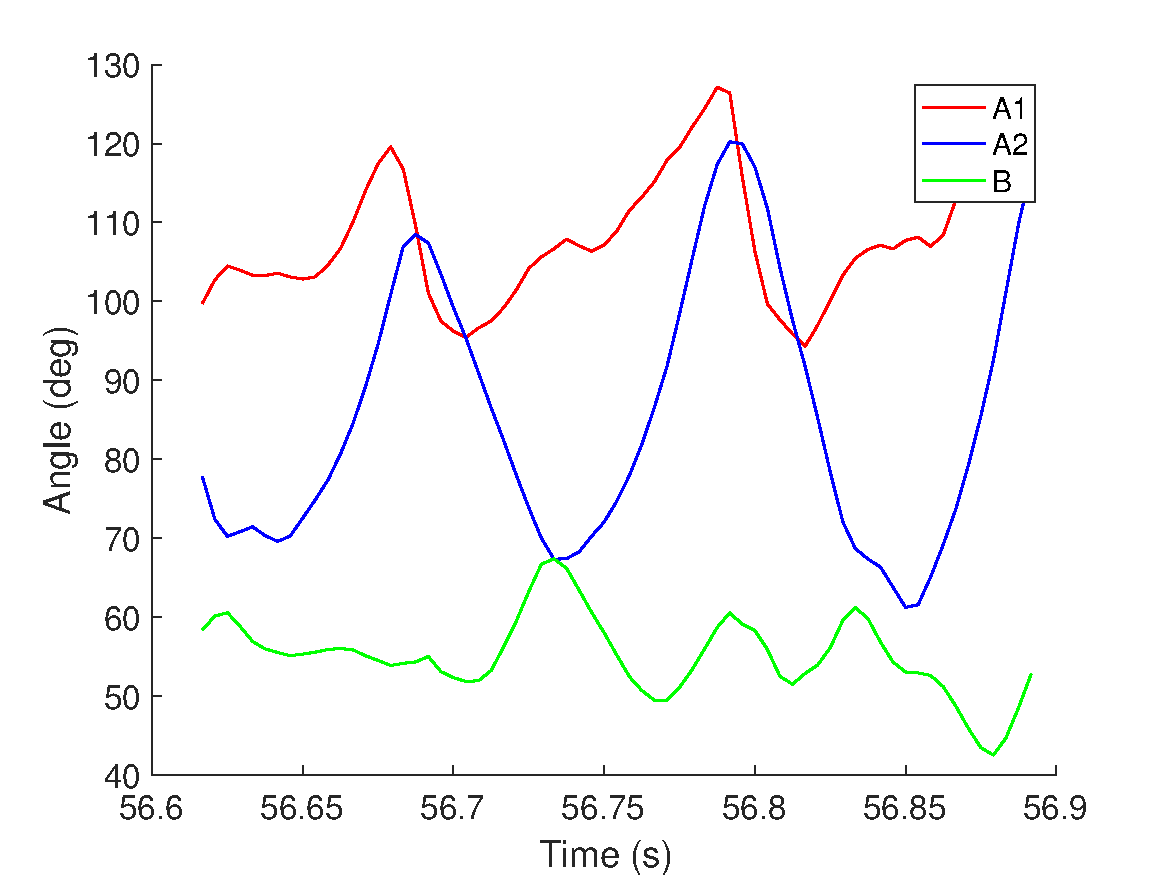
\includegraphics[width=\columnwidth]{./figure/testfig.pdf}
     \caption{キャプションを書こう}
     \label{fig:test}
\end{figure}

\begin{align}
    y=\sin{A}
    \label{eq:test}
\end{align}





%%%%%%%%%%%
% 実験
%%%%%%%%%%%
\chapter{負圧機構を有する2関節4脚壁面歩行ロボット"GeckoPath"の機構と開発}
\label{Sec:experiment}

この章ではなにをするか章の冒頭に書く

%%%%%%%%%%%%%%%%%%%%%%%%%%%%%%%%%%%%%%%%%%%%%%%%%%%%%%%%%%

\section{内部で章を分ける場合}\label{Sec:sub_experiment}

ゾウの鼻は長いぞうゾウの鼻は長いぞうゾウの鼻は長いぞうゾウの鼻は長いぞうゾウの鼻は長いぞうゾウの鼻は長いぞうゾウの鼻は長いぞうゾウの鼻は長いぞうゾウの鼻は長いぞうゾウの鼻は長いぞうゾウの鼻は長いぞうゾウの鼻は長いぞうゾウの鼻は長いぞうゾウの鼻は長いぞうゾウの鼻は長いぞうゾウの鼻は長いぞうゾウの鼻は長いぞうゾウの鼻は長いぞうゾウの鼻は長いぞうゾウの鼻は長いぞうゾウの鼻は長いぞうゾウの鼻は長いぞうゾウの鼻は長いぞうゾウの鼻は長いぞうゾウの鼻は長いぞうゾウの鼻は長いぞうゾウの鼻は長いぞうゾウの鼻は長いぞうゾウの鼻は長いぞうゾウの鼻は長いぞうゾウの鼻は長いぞうゾウの鼻は長いぞうゾウの鼻は長いぞうゾウの鼻は長いぞうゾウの鼻は長いぞうゾウの鼻は長いぞうゾウの鼻は長いぞうゾウの鼻は長いぞうゾウの鼻は長いぞうゾウの鼻は長いぞうゾウの鼻は長いぞうゾウの鼻は長いぞうゾウの鼻は長いぞうゾウの鼻は長いぞうゾウの鼻は長いぞうゾウの鼻は長いぞうゾウの鼻は長いぞうゾウの鼻は長いぞうゾウの鼻は長いぞうゾウの鼻は長いぞうゾウの鼻は長いぞうゾウの鼻は長いぞうゾウの鼻は長いぞうゾウの鼻は長いぞうゾウの鼻は長いぞうゾウの鼻は長いぞうゾウの鼻は長いぞうゾウの鼻は長いぞうゾウの鼻は長いぞうゾウの鼻は長いぞうゾウの鼻は長いぞうゾウの鼻は長いぞうゾウの鼻は長いぞうゾウの鼻は長いぞうゾウの鼻は長いぞうゾウの鼻は長いぞうゾウの鼻は長いぞうゾウの鼻は長いぞうゾウの鼻は長いぞうゾウの鼻は長いぞうゾウの鼻は長いぞうゾウの鼻は長いぞうゾウの鼻は長いぞうゾウの鼻は長いぞうゾウの鼻は長いぞうゾウの鼻は長いぞうゾウの鼻は長いぞうゾウの鼻は長いぞうゾウの鼻は長いぞうゾウの鼻は長いぞうゾウの鼻は長いぞうゾウの鼻は長いぞうゾウの鼻は長いぞうゾウの鼻は長いぞうゾウの鼻は長いぞうゾウの鼻は長いぞうゾウの鼻は長いぞうゾウの鼻は長いぞうゾウの鼻は長いぞうゾウの鼻は長いぞうゾウの鼻は長いぞうゾウの鼻は長いぞうゾウの鼻は長いぞうゾウの鼻は長いぞうゾウの鼻は長いぞうゾウの鼻は長いぞうゾウの鼻は長いぞうゾウの鼻は長いぞうゾウの鼻は長いぞうゾウの鼻は長いぞうゾウの鼻は長いぞうゾウの鼻は長いぞうゾウの鼻は長いぞうゾウの鼻は長いぞうゾウの鼻は長いぞうゾウの鼻は長いぞうゾウの鼻は長いぞうゾウの鼻は長いぞうゾウの鼻は長いぞうゾウの鼻は長いぞうゾウの鼻は長いぞうゾウの鼻は長いぞうゾウの鼻は長いぞうゾウの鼻は長いぞうゾウの鼻は長いぞうゾウの鼻は長いぞうゾウの鼻は長いぞうゾウの鼻は長いぞうゾウの鼻は長いぞうゾウの鼻は長いぞうゾウの鼻は長いぞうゾウの鼻は長いぞうゾウの鼻は長いぞうゾウの鼻は長いぞうゾウの鼻は長いぞうゾウの鼻は長いぞうゾウの鼻は長いぞうゾウの鼻は長いぞうゾウの鼻は長いぞうゾウの鼻は長いぞうゾウの鼻は長いぞうゾウの鼻は長いぞうゾウの鼻は長いぞうゾウの鼻は長いぞうゾウの鼻は長いぞうゾウの鼻は長いぞうゾウの鼻は長いぞうゾウの鼻は長いぞうゾウの鼻は長いぞうゾウの鼻は長いぞうゾウの鼻は長いぞうゾウの鼻は長いぞうゾウの鼻は長いぞうゾウの鼻は長いぞうゾウの鼻は長いぞうゾウの鼻は長いぞうゾウの鼻は長いぞうゾウの鼻は長いぞうゾウの鼻は長いぞうゾウの鼻は長いぞうゾウの鼻は長いぞうゾウの鼻は長いぞうゾウの鼻は長いぞうゾウの鼻は長いぞうゾウの鼻は長いぞうゾウの鼻は長いぞうゾウの鼻は長いぞうゾウの鼻は長いぞうゾウの鼻は長いぞうゾウの鼻は長いぞうゾウの鼻は長いぞうゾウの鼻は長いぞうゾウの鼻は長いぞうゾウの鼻は長いぞうゾウの鼻は長いぞうゾウの鼻は長いぞうゾウの鼻は長いぞうゾウの鼻は長いぞうゾウの鼻は長いぞうゾウの鼻は長いぞうゾウの鼻は長いぞうゾウの鼻は長いぞうゾウの鼻は長いぞうゾウの鼻は長いぞうゾウの鼻は長いぞうゾウの鼻は長いぞうゾウの鼻は長いぞうゾウの鼻は長いぞうゾウの鼻は長いぞうゾウの鼻は長いぞうゾウの鼻は長いぞうゾウの鼻は長いぞうゾウの鼻は長いぞうゾウの鼻は長いぞうゾウの鼻は長いぞうゾウの鼻は長いぞうゾウの鼻は長いぞうゾウの鼻は長いぞうゾウの鼻は長いぞうゾウの鼻は長いぞうゾウの鼻は長いぞうゾウの鼻は長いぞうゾウの鼻は長いぞうゾウの鼻は長いぞうゾウの鼻は長いぞうゾウの鼻は長いぞうゾウの鼻は長いぞうゾウの鼻は長いぞうゾウの鼻は長いぞうゾウの鼻は長いぞうゾウの鼻は長いぞうゾウの鼻は長いぞうゾウの鼻は長いぞうゾウの鼻は長いぞうゾウの鼻は長いぞうゾウの鼻は長いぞうゾウの鼻は長いぞうゾウの鼻は長いぞうゾウの鼻は長いぞうゾウの鼻は長いぞうゾウの鼻は長いぞうゾウの鼻は長いぞうゾウの鼻は長いぞうゾウの鼻は長いぞうゾウの鼻は長いぞうゾウの鼻は長いぞうゾウの鼻は長いぞうゾウの鼻は長いぞうゾウの鼻は長いぞうゾウの鼻は長いぞうゾウの鼻は長いぞうゾウの鼻は長いぞうゾウの鼻は長いぞうゾウの鼻は長いぞうゾウの鼻は長いぞうゾウの鼻は長いぞうゾウの鼻は長いぞうゾウの鼻は長いぞうゾウの鼻は長いぞうゾウの鼻は長いぞうゾウの鼻は長いぞうゾウの鼻は長いぞうゾウの鼻は長いぞうゾウの鼻は長いぞうゾウの鼻は長いぞうゾウの鼻は長いぞうゾウの鼻は長いぞうゾウの鼻は長いぞうゾウの鼻は長いぞうゾウの鼻は長いぞうゾウの鼻は長いぞうゾウの鼻は長いぞうゾウの鼻は長いぞうゾウの鼻は長いぞうゾウの鼻は長いぞうゾウの鼻は長いぞうゾウの鼻は長いぞうゾウの鼻は長いぞうゾウの鼻は長いぞうゾウの鼻は長いぞうゾウの鼻は長いぞうゾウの鼻は長いぞうゾウの鼻は長いぞうゾウの鼻は長いぞうゾウの鼻は長いぞうゾウの鼻は長いぞうゾウの鼻は長いぞうゾウの鼻は長いぞうゾウの鼻は長いぞうゾウの鼻は長いぞうゾウの鼻は長いぞうゾウの鼻は長いぞうゾウの鼻は長いぞうゾウの鼻は長いぞうゾウの鼻は長いぞうゾウの鼻は長いぞうゾウの鼻は長いぞうゾウの鼻は長いぞうゾウの鼻は長いぞうゾウの鼻は長いぞうゾウの鼻は長いぞうゾウの鼻は長いぞうゾウの鼻は長いぞうゾウの鼻は長いぞうゾウの鼻は長いぞうゾウの鼻は長いぞうゾウの鼻は長いぞうゾウの鼻は長いぞうゾウの鼻は長いぞうゾウの鼻は長いぞうゾウの鼻は長いぞうゾウの鼻は長いぞうゾウの鼻は長いぞうゾウの鼻は長いぞうゾウの鼻は長いぞうゾウの鼻は長いぞうゾウの鼻は長いぞうゾウの鼻は長いぞうゾウの鼻は長いぞうゾウの鼻は長いぞうゾウの鼻は長いぞうゾウの鼻は長いぞうゾウの鼻は長いぞうゾウの鼻は長いぞうゾウの鼻は長いぞうゾウの鼻は長いぞうゾウの鼻は長いぞうゾウの鼻は長いぞうゾウの鼻は長いぞうゾウの鼻は長いぞうゾウの鼻は長いぞうゾウの鼻は長いぞうゾウの鼻は長いぞうゾウの鼻は長いぞうゾウの鼻は長いぞうゾウの鼻は長いぞうゾウの鼻は長いぞうゾウの鼻は長いぞうゾウの鼻は長いぞうゾウの鼻は長いぞうゾウの鼻は長いぞうゾウの鼻は長いぞうゾウの鼻は長いぞうゾウの鼻は長いぞうゾウの鼻は長いぞうゾウの鼻は長いぞうゾウの鼻は長いぞうゾウの鼻は長いぞうゾウの鼻は長いぞうゾウの鼻は長いぞうゾウの鼻は長いぞうゾウの鼻は長いぞうゾウの鼻は長いぞうゾウの鼻は長いぞうゾウの鼻は長いぞうゾウの鼻は長いぞうゾウの鼻は長いぞうゾウの鼻は長いぞうゾウの鼻は長いぞうゾウの鼻は長いぞうゾウの鼻は長いぞうゾウの鼻は長いぞうゾウの鼻は長いぞうゾウの鼻は長いぞうゾウの鼻は長いぞうゾウの鼻は長いぞうゾウの鼻は長いぞうゾウの鼻は長いぞうゾウの鼻は長いぞうゾウの鼻は長いぞうゾウの鼻は長いぞうゾウの鼻は長いぞうゾウの鼻は長いぞうゾウの鼻は長いぞうゾウの鼻は長いぞうゾウの鼻は長いぞうゾウの鼻は長いぞうゾウの鼻は長いぞうゾウの鼻は長いぞうゾウの鼻は長いぞうゾウの鼻は長いぞうゾウの鼻は長いぞうゾウの鼻は長いぞうゾウの鼻は長いぞうゾウの鼻は長いぞうゾウの鼻は長いぞうゾウの鼻は長いぞうゾウの鼻は長いぞうゾウの鼻は長いぞうゾウの鼻は長いぞうゾウの鼻は長いぞうゾウの鼻は長いぞうゾウの鼻は長いぞうゾウの鼻は長いぞうゾウの鼻は長いぞうゾウの鼻は長いぞうゾウの鼻は長いぞうゾウの鼻は長いぞうゾウの鼻は長いぞうゾウの鼻は長いぞうゾウの鼻は長いぞうゾウの鼻は長いぞうゾウの鼻は長いぞうゾウの鼻は長いぞうゾウの鼻は長いぞうゾウの鼻は長いぞうゾウの鼻は長いぞうゾウの鼻は長いぞうゾウの鼻は長いぞうゾウの鼻は長いぞうゾウの鼻は長いぞうゾウの鼻は長いぞうゾウの鼻は長いぞうゾウの鼻は長いぞうゾウの鼻は長いぞうゾウの鼻は長いぞうゾウの鼻は長いぞうゾウの鼻は長いぞうゾウの鼻は長いぞうゾウの鼻は長いぞうゾウの鼻は長いぞうゾウの鼻は長いぞうゾウの鼻は長いぞうゾウの鼻は長いぞうゾウの鼻は長いぞうゾウの鼻は長いぞうゾウの鼻は長いぞうゾウの鼻は長いぞうゾウの鼻は長いぞうゾウの鼻は長いぞうゾウの鼻は長いぞうゾウの鼻は長いぞうゾウの鼻は長いぞうゾウの鼻は長いぞうゾウの鼻は長いぞうゾウの鼻は長いぞうゾウの鼻は長いぞうゾウの鼻は長いぞうゾウの鼻は長いぞうゾウの鼻は長いぞうゾウの鼻は長いぞうゾウの鼻は長いぞうゾウの鼻は長いぞうゾウの鼻は長いぞうゾウの鼻は長いぞうゾウの鼻は長いぞうゾウの鼻は長いぞうゾウの鼻は長いぞうゾウの鼻は長いぞうゾウの鼻は長いぞうゾウの鼻は長いぞうゾウの鼻は長いぞうゾウの鼻は長いぞうゾウの鼻は長いぞうゾウの鼻は長いぞうゾウの鼻は長いぞうゾウの鼻は長いぞうゾウの鼻は長いぞうゾウの鼻は長いぞうゾウの鼻は長いぞうゾウの鼻は長いぞうゾウの鼻は長いぞうゾウの鼻は長いぞうゾウの鼻は長いぞうゾウの鼻は長いぞうゾウの鼻は長いぞうゾウの鼻は長いぞうゾウの鼻は長いぞうゾウの鼻は長いぞうゾウの鼻は長いぞうゾウの鼻は長いぞうゾウの鼻は長いぞうゾウの鼻は長いぞうゾウの鼻は長いぞうゾウの鼻は長いぞうゾウの鼻は長いぞうゾウの鼻は長いぞうゾウの鼻は長いぞうゾウの鼻は長いぞうゾウの鼻は長いぞうゾウの鼻は長いぞうゾウの鼻は長いぞうゾウの鼻は長いぞうゾウの鼻は長いぞうゾウの鼻は長いぞうゾウの鼻は長いぞうゾウの鼻は長いぞうゾウの鼻は長いぞうゾウの鼻は長いぞうゾウの鼻は長いぞうゾウの鼻は長いぞうゾウの鼻は長いぞうゾウの鼻は長いぞうゾウの鼻は長いぞうゾウの鼻は長いぞうゾウの鼻は長いぞうゾウの鼻は長いぞうゾウの鼻は長いぞうゾウの鼻は長いぞうゾウの鼻は長いぞうゾウの鼻は長いぞうゾウの鼻は長いぞうゾウの鼻は長いぞうゾウの鼻は長いぞうゾウの鼻は長いぞうゾウの鼻は長いぞうゾウの鼻は長いぞうゾウの鼻は長いぞうゾウの鼻は長いぞうゾウの鼻は長いぞうゾウの鼻は長いぞうゾウの鼻は長いぞうゾウの鼻は長いぞうゾウの鼻は長いぞうゾウの鼻は長いぞうゾウの鼻は長いぞうゾウの鼻は長いぞうゾウの鼻は長いぞうゾウの鼻は長いぞうゾウの鼻は長いぞうゾウの鼻は長いぞうゾウの鼻は長いぞうゾウの鼻は長いぞうゾウの鼻は長いぞうゾウの鼻は長いぞうゾウの鼻は長いぞうゾウの鼻は長いぞうゾウの鼻は長いぞうゾウの鼻は長いぞうゾウの鼻は長いぞうゾウの鼻は長いぞうゾウの鼻は長いぞうゾウの鼻は長いぞうゾウの鼻は長いぞうゾウの鼻は長いぞうゾウの鼻は長いぞうゾウの鼻は長いぞうゾウの鼻は長いぞうゾウの鼻は長いぞうゾウの鼻は長いぞうゾウの鼻は長いぞうゾウの鼻は長いぞうゾウの鼻は長いぞうゾウの鼻は長いぞうゾウの鼻は長いぞうゾウの鼻は長いぞうゾウの鼻は長いぞうゾウの鼻は長いぞうゾウの鼻は長いぞうゾウの鼻は長いぞうゾウの鼻は長いぞうゾウの鼻は長いぞうゾウの鼻は長いぞうゾウの鼻は長いぞうゾウの鼻は長いぞうゾウの鼻は長いぞうゾウの鼻は長いぞうゾウの鼻は長いぞうゾウの鼻は長いぞうゾウの鼻は長いぞうゾウの鼻は長いぞうゾウの鼻は長いぞうゾウの鼻は長いぞうゾウの鼻は長いぞうゾウの鼻は長いぞうゾウの鼻は長いぞうゾウの鼻は長いぞうゾウの鼻は長いぞうゾウの鼻は長いぞうゾウの鼻は長いぞうゾウの鼻は長いぞうゾウの鼻は長いぞうゾウの鼻は長いぞうゾウの鼻は長いぞうゾウの鼻は長いぞうゾウの鼻は長いぞうゾウの鼻は長いぞうゾウの鼻は長いぞうゾウの鼻は長いぞうゾウの鼻は長いぞうゾウの鼻は長いぞうゾウの鼻は長いぞうゾウの鼻は長いぞうゾウの鼻は長いぞうゾウの鼻は長いぞうゾウの鼻は長いぞうゾウの鼻は長いぞうゾウの鼻は長いぞうゾウの鼻は長いぞうゾウの鼻は長いぞうゾウの鼻は長いぞうゾウの鼻は長いぞうゾウの鼻は長いぞうゾウの鼻は長いぞうゾウの鼻は長いぞうゾウの鼻は長いぞうゾウの鼻は長いぞうゾウの鼻は長いぞうゾウの鼻は長いぞうゾウの鼻は長いぞうゾウの鼻は長いぞうゾウの鼻は長いぞうゾウの鼻は長いぞうゾウの鼻は長いぞうゾウの鼻は長いぞうゾウの鼻は長いぞうゾウの鼻は長いぞうゾウの鼻は長いぞうゾウの鼻は長いぞうゾウの鼻は長いぞうゾウの鼻は長いぞうゾウの鼻は長いぞうゾウの鼻は長いぞうゾウの鼻は長いぞうゾウの鼻は長いぞうゾウの鼻は長いぞうゾウの鼻は長いぞうゾウの鼻は長いぞうゾウの鼻は長いぞうゾウの鼻は長いぞうゾウの鼻は長いぞうゾウの鼻は長いぞうゾウの鼻は長いぞうゾウの鼻は長いぞうゾウの鼻は長いぞうゾウの鼻は長いぞうゾウの鼻は長いぞうゾウの鼻は長いぞうゾウの鼻は長いぞうゾウの鼻は長いぞうゾウの鼻は長いぞうゾウの鼻は長いぞうゾウの鼻は長いぞうゾウの鼻は長いぞうゾウの鼻は長いぞうゾウの鼻は長いぞうゾウの鼻は長いぞうゾウの鼻は長いぞうゾウの鼻は長いぞうゾウの鼻は長いぞうゾウの鼻は長いぞうゾウの鼻は長いぞうゾウの鼻は長いぞうゾウの鼻は長いぞうゾウの鼻は長いぞうゾウの鼻は長いぞうゾウの鼻は長いぞうゾウの鼻は長いぞうゾウの鼻は長いぞうゾウの鼻は長いぞうゾウの鼻は長いぞうゾウの鼻は長いぞうゾウの鼻は長いぞうゾウの鼻は長いぞうゾウの鼻は長いぞうゾウの鼻は長いぞうゾウの鼻は長いぞうゾウの鼻は長いぞうゾウの鼻は長いぞうゾウの鼻は長いぞうゾウの鼻は長いぞうゾウの鼻は長いぞうゾウの鼻は長いぞうゾウの鼻は長いぞうゾウの鼻は長いぞうゾウの鼻は長いぞうゾウの鼻は長いぞうゾウの鼻は長いぞうゾウの鼻は長いぞうゾウの鼻は長いぞうゾウの鼻は長いぞうゾウの鼻は長いぞうゾウの鼻は長いぞうゾウの鼻は長いぞうゾウの鼻は長いぞうゾウの鼻は長いぞうゾウの鼻は長いぞうゾウの鼻は長いぞうゾウの鼻は長いぞうゾウの鼻は長いぞうゾウの鼻は長いぞうゾウの鼻は長いぞうゾウの鼻は長いぞうゾウの鼻は長いぞうゾウの鼻は長いぞうゾウの鼻は長いぞうゾウの鼻は長いぞうゾウの鼻は長いぞうゾウの鼻は長いぞうゾウの鼻は長いぞうゾウの鼻は長いぞうゾウの鼻は長いぞうゾウの鼻は長いぞうゾウの鼻は長いぞうゾウの鼻は長いぞうゾウの鼻は長いぞうゾウの鼻は長いぞうゾウの鼻は長いぞうゾウの鼻は長いぞうゾウの鼻は長いぞうゾウの鼻は長いぞうゾウの鼻は長いぞうゾウの鼻は長いぞうゾウの鼻は長いぞうゾウの鼻は長いぞうゾウの鼻は長いぞうゾウの鼻は長いぞうゾウの鼻は長いぞうゾウの鼻は長いぞうゾウの鼻は長いぞうゾウの鼻は長いぞうゾウの鼻は長いぞうゾウの鼻は長いぞうゾウの鼻は長いぞうゾウの鼻は長いぞうゾウの鼻は長いぞうゾウの鼻は長いぞうゾウの鼻は長いぞうゾウの鼻は長いぞうゾウの鼻は長いぞうゾウの鼻は長いぞうゾウの鼻は長いぞうゾウの鼻は長いぞうゾウの鼻は長いぞうゾウの鼻は長いぞうゾウの鼻は長いぞうゾウの鼻は長いぞうゾウの鼻は長いぞうゾウの鼻は長いぞうゾウの鼻は長いぞうゾウの鼻は長いぞうゾウの鼻は長いぞうゾウの鼻は長いぞうゾウの鼻は長いぞうゾウの鼻は長いぞうゾウの鼻は長いぞうゾウの鼻は長いぞうゾウの鼻は長いぞうゾウの鼻は長いぞうゾウの鼻は長いぞうゾウの鼻は長いぞうゾウの鼻は長いぞうゾウの鼻は長いぞうゾウの鼻は長いぞうゾウの鼻は長いぞうゾウの鼻は長いぞうゾウの鼻は長いぞうゾウの鼻は長いぞうゾウの鼻は長いぞうゾウの鼻は長いぞう

%%%%%%%%%%%
% 結果
%%%%%%%%%%%

この章ではなにをするか章の冒頭に書く

%\input{contents/3/3-1.tex}%このようにしてソースファイルを分割しても良い
%\newpage

%\input{contents/3/3-2.tex}
%\newpage
%%%%%%%%%%%%%%%%%%%%%%%%%%%%%%%%%%%%%%%%%%%%%%%%%%%%%%%%%%%%%

%%%%%%%%%%%%%%%%%%%%%%%%%%%%%%%%%%%%%%%%%%%%%%%%%%%%%%%%%%%%%


%%%%%%%%%%%
% 結言
%%%%%%%%%%%
\chapter{結言}
\label{Sec:conclusion}


%%%%%%%%%%%%%%%%%%%%%%%%%%%%%%%%%%%%%%%%%%%%%%%%%%%%%%%%%%%%
%
%後書き
\backmatter
%
%%%%%%%%%%%%%%%%%%%%%%%%%%%%%%%%%%%%%%%%%%%%%%%%%%%%%%%%%%%%
%謝辞
\chapter*{謝辞}
\thispagestyle{empty}
%%%%%%%
% 謝辞
%%%%%%%
謝辞を書こう
ボケる必要はない
%%%%%%%%%%%%%%%%%%%%%%%%%%%%%%%%%%%%%%%%%%%%%%%%%%%%%%%%%%%%


%%%%%%%%%%%%
% 参考文献
%%%%%%%%%%%%
\bibliographystyle{osukalab_bibstyle}             % 参考文献
\bibliography{myref}                       % myref.bib にデータを登録

\end{document}
